\subsection{Results}

\begin{itemize}
    \item Question: What is the calculated diffusion constant? How does it compare to the experimental value of 2.43 times 10-5 cm2 div s?
\end{itemize}

The calculated diffusion constant is 2.5681 (+/- 0.1929) 10-5 cm^2/s. Including the margin of error this result is as excepted. 

The diffsion coefficient the quantity of a substance that in diffusing from one region to another passes through each unit of cross section per unit of time when the volume-concentration gradient is unity—called also diffusivity.       
        

\begin{figure}[t]
    \centering
    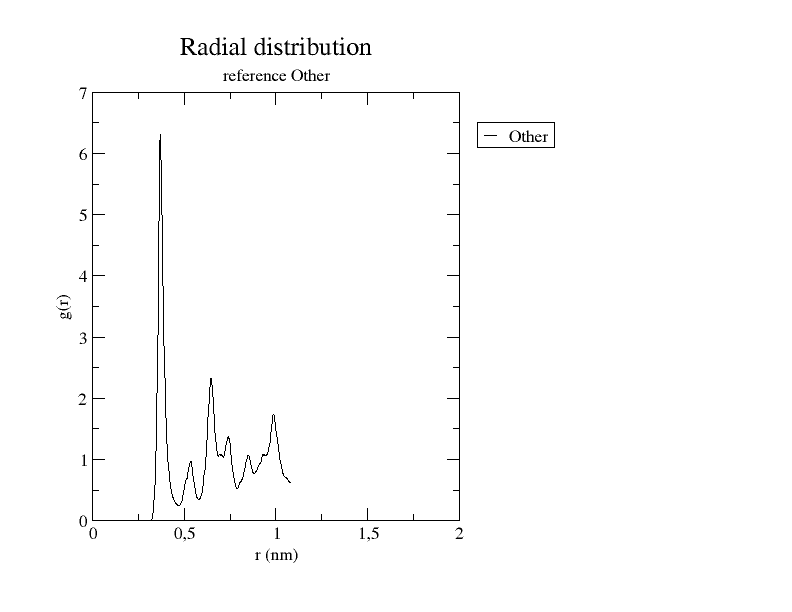
\includegraphics[width=180px]{plots/rdf_solid.png}
    \caption{Figure rdf from solid argon; correlation function against distance}
    \label{rdf solid}
\end{figure}

\begin{figure}[t]
    \centering
    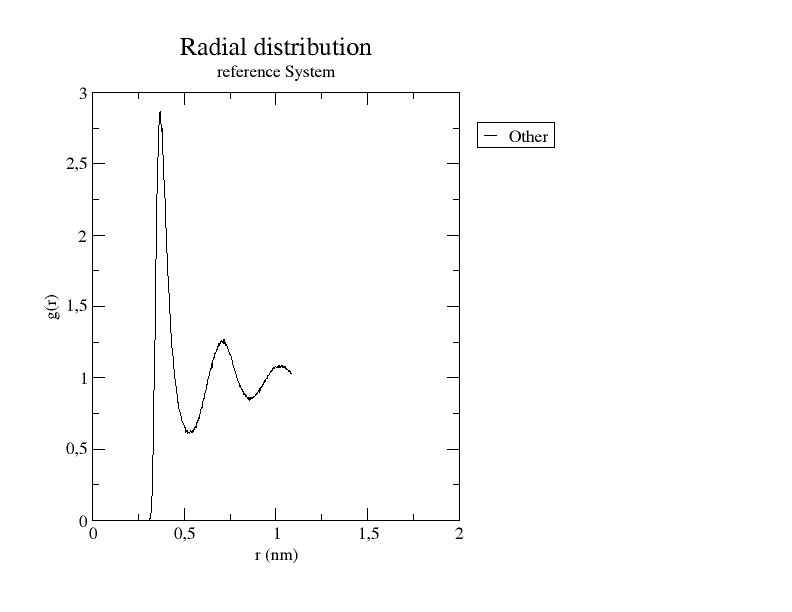
\includegraphics[width=180px]{plots/rdf_liquid.png}
    \caption{Figure rdf from solid argon; correlation function against distance}
    \label{rdf liquid}
\end{figure}

At both rdf before 0.3 there is zero correlation. The first peak is at r=0.37nm and g(r)=2.85 for liquid argon und g(r)=6.30 for solid argon, these are the highest peaks for each plot. In the liquid plot the next peak at 0.71nm. In the rdf plot for solid argon there is a small peak at r=0.54 with g(r) = 0.97 and a higher peak with g(r)=2.23 at r=0.65.

g(r) corrolation function, relation from bulk density(=average density) to local density(density from one molecule to an other) discribes the variation in density as a function of distance, so higher g(r) means more molecules at r.

Nearing r<3 the rdf is 0 as well for both states. This can be explained by the Lennard-Jones-Potential, because of the repulsion no two molecules are at close distance. The most molecules are at r=0.37, corresponding to the minimun in the LJP and experimental findings [QUELLEN].
In solid state the peaks are higher and well defined, because the atoms are densly packed. The second (high > 0) peak appears at r=0.65 wich is roughly twice the distance from the center. This shows the constant structure of the solid phase. The broadening of the shape is because of vibrating of the molecules.In comparison the rdf of liquid argon shows the first peak ate the same r, but g(r) is half the size, which means less atoms at this given distance. The second peak is not at twice the distance as the first. Liquids are moore loosely packed so the intervals aren't as exact as in solids.

%http://www.sklogwiki.org/SklogWiki/index.php/Argon
%https://www.ncbi.nlm.nih.gov/pmc/articles/PMC349093/?page=4